\documentclass[a4paper]{article}

%% Language and font encodings
\usepackage[english]{babel}
\usepackage[utf8]{inputenc}
\usepackage[T1]{fontenc}
\usepackage{textcomp}

\usepackage{booktabs}
\usepackage{tabu}
\usepackage[T1]{fontenc}

%% Sets page size and margins
\usepackage[a4paper,top=3cm,bottom=2cm,left=3cm,right=3cm,marginparwidth=1.75cm]{geometry}

%% Useful packages
\usepackage{amsmath}
\usepackage{graphicx}
%\usepackage{apacite}
\usepackage[colorinlistoftodos]{todonotes}
\usepackage[colorlinks=true, allcolors=blue]{hyperref}
\usepackage[backend=bibtex]{biblatex}
%\bibliographystyle{plain}
\addbibresource{My_Collection.bib}

\title{Synchronisation of Subtitle Track with Recorded Audio}
\author{Joshua Fenech}
%\date{}

\begin{document}
\maketitle

\section{Aim}
To synchronise a time indexed subtitle track with a video using independent audio input in a real setting, (i.e. in a cinema), so that a phone can be used to display the subtitles based on recording the sound via a microphone. The model would be trained using the original sound file but would be tested using noisy output, therefore a means of incorporating robustness would be prioritised.

\section{Background}
A study was undertaken to perform subtitle synchronisation by \cite{sabater_2017}. In this approach, the aim is to perform the synchronisation on the original data, i.e. the movie file itself, and has no intention of deploying this in noisy real world settings. The approach is to extract the audio at 16kHz in order to capture human speech. The audio is then preprocessed using Mel Frequency Cepstral Coefficient, which assumes that the audio barely changes in small frames (20-40ms). For each frame, MFCC calculates the periodogram that contains information on the frequencies present and their relevant importance in terms of energy. This result is processed further by taking logarithms and applying a Discrete Cosine Transform in order to obtain 2-13 coefficients representing the most important features of each audiogram.

In order to interpret this data as a classification problem, the author used as input the MFCC features extracted from the audio, and as output the synchronised subtitle files indicate whether someone is speaking (value 1) or not (value 0). A recurrent neural network was then used to take the input, and return a probability of having a subtitle in the period of time represented by input samples. When trained on all the audiograms, the result is an array of probabilities that consecutively represent finding speech in the associated time frame.

\begin{figure}[h]
	\centering
	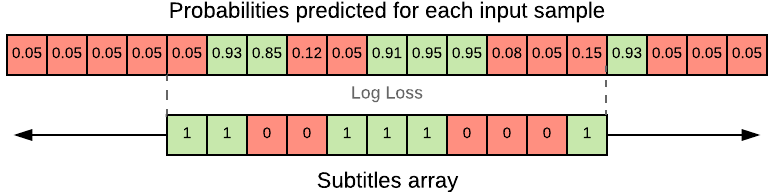
\includegraphics[scale=0.5]{prob_array.png}
	\caption{Sourced from https://machinelearnings.co/automatic-subtitle-synchronization-e188a9275617}
\end{figure}

By taking a window of n audiograms, a log loss function was used to correlate the audio with the subtitles, and from this the position is identified and the subtitles can be synchronised.

This approached achieved an accuracy of ± 0.064s, and with the use of dynamic programming completed synchronisation in 45 seconds. This is a satisfactory result but is only applicable in a perfect, noiseless setting, and may not function in the realworld setting. Further issues are that this is not in real time, whereby a signal is received and the audiograms must be identified and from this the correct location in the subtitle track found in order to enable synchronisation. Differences in location of the microphone (seat), possible subtle differences in exact film distribution and other variations need also be taken into account.

Other papers have examined the use of subtitle tracks as a means of associating characters to speech by comparing the subtitle track with the script \cite{Everingham2006}, for identifying actions in video using a similar method \cite{Cour2008}. A further development of this was performed \cite{K2009} which used the video itself in order to identify features to align a movie to script for use in cases where subtitle tracks are not available. A python module is available on github for correlating 2 audiofiles in order to add the subtitle timings from one track to the other, but again relies on possession of a second full recording and not in real time.

\section{Tasks}
It will be necessary to generate noisy audio datasets that already have subtitle tracks. This could be done by manually recording the films. Although this would take some hours, the nature of the sampling would generate many thousands of samples on which to train on, and would not take much active involvement. Different microphones and positions could be used to include more variation. A second method would be to digitally introduce noise by convolution, which would allow more freedom but care would be needed to find a representative form of noise to use (a simple gaussian function would be inappropriate).

Once this has been generated, the audio signal would need to be preprocessed in order to take account of this noise, the filter for which would need to be investigated. A similar approach could then be taken by Sabater, but due to the real time nature, would need to be adapted in order to store a specific period of audio input and correlate this, whilst taking into account that the processing time would need to be incorporated into the model. Hidden Markov Models may be appropriate due to the sequential nature, with a go-back-n type implementation. The processing requirements would need to be analysed with the intention that at least the process of using the trained model can be operated on a mobile device.

%\input{paper}

\printbibliography
\end{document}